%%% Preamble
\documentclass[DIV=calc,paper=a4,fontsize=9pt,twocolumn]{scrartcl}
\renewcommand*\sfdefault{lcmss}
\renewcommand*\familydefault{\sfdefault} %% Only if the base font of the document is to be sans serif
\usepackage[T1]{fontenc}

\usepackage{lipsum}                                                 
\usepackage[utf8x]{inputenc}
\usepackage[english]{babel}								% English language/hyphenation
\usepackage[protrusion=true,expansion=true]{microtype}	% Better typography
\usepackage{amsmath,amsfonts,amsthm}					% Math packages
\usepackage[pdftex]{graphicx}							% Enable pdflatex
\usepackage[svgnames]{xcolor}							% Enabling colors by their 'svgnames'

\usepackage{epstopdf}									% Converts .eps to .pdf
\usepackage{subfig}										% Subfigures
\usepackage{booktabs}									% Nicer tables
\usepackage{fix-cm}										% Custom fontsizes
\usepackage{csquotes}
\usepackage[authoryear,round]{natbib}
\usepackage{float}
\bibliographystyle{natdin}
\definecolor{headblue}{HTML}{15778E}
\definecolor{borderblue}{HTML}{074C5C}

%%% Custom sectioning (sectsty package)
\usepackage{sectsty}		
							% Custom sectioning (see below)
\allsectionsfont{\usefont{OT1}{phv}{b}{n}}				% Change font of al section commands
														% bch-b-n: CharterBT-Bold font

\sectionfont{\usefont{OT1}{phv}{b}{n}}					% Change font of \section command
														% bch-b-n: CharterBT-Bold font



%%% Headers and footers
\usepackage{fancyhdr}									% Needed to define custom headers/footers
    \pagestyle{fancy}									% Enabling the custom headers/footers
\usepackage{lastpage}   

% Header (empty)
\lhead{}
\chead{}
\rhead{}
% Footer (you may change this to your own needs)
\lfoot{\footnotesize 2013 \textbullet ~ Tools and Evaluation Methods used in Open Source Development}
\cfoot{}
\rfoot{\footnotesize page \thepage\ of \pageref{LastPage}}  % "Page 1 of 2"
\renewcommand{\headrulewidth}{0.0pt}
\renewcommand{\footrulewidth}{0.4pt}



%%% Creating an initial of the very first character of the content
\usepackage{lettrine}
\newcommand{\initial}[1]{%
     \lettrine[lines=2,lhang=0.3,nindent=0em]{
                    \color{headblue}
                    {\textsf{#1}}}{}}



%%% Title, author and date metadata
\usepackage{titling}										% For custom titles

\newcommand{\HorRule}{\color{headblue}\rule{\linewidth}{1pt}}

\pretitle{\vspace{-30pt} \begin{flushleft}  \fontsize{30}{30} \usefont{OT1}{phv}{b}{n} \color{borderblue} \selectfont }
\title{Tools and Evaluation Methods used in Open Source Development}    % Title of your article goes here
\posttitle{\par\end{flushleft}\vskip 0.5em}

\preauthor{\begin{flushleft} \large \usefont{OT1}{phv}{b}{sl} \color{headblue}}
\author{Steffen Tröster \\}											% Author name goes here
\postauthor{\footnotesize \usefont{OT1}{phv}{m}{sl} \color{Black} 
                    University of Tampere, 2013							% Institution of author
                    \par\end{flushleft}\HorRule}

\date{}																% No date



%%% Begin document
\begin{document}
\maketitle
\thispagestyle{fancy}		% Enabling the custom headers/footers for the first page 
% The first character should be within \initial{}
\initial{O}ne says that the open source paradigm is one of the most promising strategies to improve the quality and efficiency of software development processes. This essay is introducing into the paradigm of open source, its software development model and its use of software engineering tools during the processes.

% After this introducing part the essay will review an evaluation of the open source paradigm by \citet{fuggetta2003open} and will try to show up typically evaluation properties with affiliated measurements.

\section{Introduction}

The open source software development paradigm is one of the most upcoming way of new software development. Software developed in this way is free in use, spreading and contribution with the condition of continuing the open source paradigm. But this \enquote{free} results out of open source development processes are nearly all commercial projects with service opportunities \citep{Wheeler}.

To ensure a proper result in open source development with all different co-developer, from an established community, there should be a sharp regulation progress for input and iterations. Also difficult is the opportunity to develop from everywhere in the world. Therefor the open source development paradigm uses a set of different software engineering tools with features which helps the given in cases like collaboration, status-tracking and testing.

\enquote{To a large extent, the open source culture and methodology are conveyed to new developers via the toolset itself, and through the demonstrated usage of these tools on existing projects.} \citep{Robbins02adoptingoss}

There are different indicators why open source is one of the most promising strategies to improve the quality and efficiency of software development processes. The first one is that projects have a huge crowd of individual users who are willing to contribute to a project by different impulsions. This causes fresh ideas and resources. Thats why companies are more and more focusing on the open source approach. They can successfully develop bigger projects by involving the community. But also public institutions are as even interested on this approach. Open Source can form more security, safety and trustworthiness this division because everyone can check and view the used systems. The last indicator are popular and successful products like \enquote{Linux} and \enquote{Apache} which are gaining more and more shares in their own markets. \citep{fuggetta2003open}

\subsection{Open Source Software Development Model}

Next to the given toolset, there is an Open Source Development Model which is characterized by processes and values of a different kind as traditional proprietary development models. This model takes a new approach for more fluidly development by increasing collaboration, continuous integration and testing. It also involves the end-users deeper into design decisions. Some companies may use a slightly modified version of this model depending on their claims. \citep{Haddad11}

The Model in Figure \ref{fig:feature-life-cycle} shows a typical feature life-cycle. A feature request is coming from the user or developer community of the project by mailing list or issue tracker. It will discussed in the whole community and results to an architecture or design decision which is received into to implementation process if it is accepted. The new feature will after the implementation verified by continuous integration and (automated) testing. This whole process is iteration based and can flow back to the decision process to ensure a necessary project quality when for example a testing of a feature failed and when it contradicts other design decisions. After a successfully testing the feature will be deployed in a new project version and can be maintenanced by the user and development community. \citep{Haddad11}

\begin{figure*}[ht]
    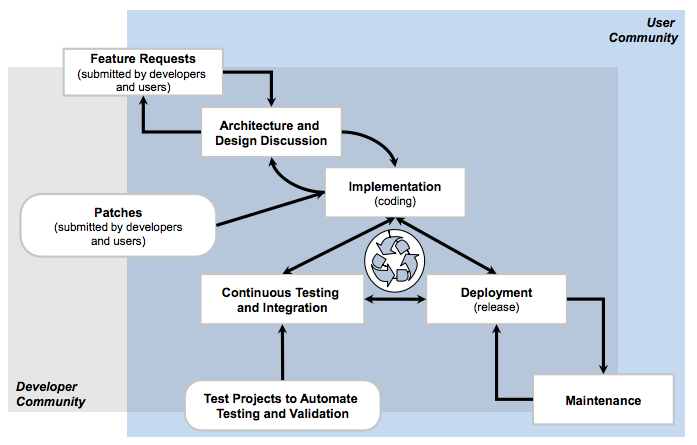
\includegraphics[width=0.8\textwidth ]{img/feature-life-cycle.png}{}
    \centering
    \caption{Feature life-cycle in the open source development model. \citet{Haddad11}}\label{fig:feature-life-cycle}
\end{figure*}

\section{Tools in Open Source Software Development}

Software Engineering tools which are created and used in open source software development are fitting to the different processes of the given software development model. These tools are widly the result of daily practices so that they carry support for the given use cases in open source software development. \citep{Robbins02adoptingoss} 

Back to the model of \citet{Haddad11}, each process is constituting a special type of tool. First of all communication tools are important to contribute feature requests, issues and bugs to a project. These tools are also used to make the design decisions in the developer and user community. The second topic of tools are version control systems and collaboration tools to facilitate parallel contribution from all over the world. The software need to be tested according to the given open source model after contribution. Therefor a toolset of different testing and continues integration tools are available. They will be discussed in the following sub chapters.

\subsection{Communication - Issue and Bugtracking}

The most important action, which is done in every process of the open source software development model is communication. Almost every project is using mailing lists to discuss design decisions and new features and approaches with the developer and user community. Some projects are using asynchrounus communication like IRC in addition, but it is still a more or less organized communication process. Next to these direct communication techniques, there are are also the projects websites, FAQ's and Wikis in use to communicate news and important information about the project to users which are not participating. \citep{ApacheFoundation13} 

An even more organized communication are offering issue-tracker or ticket-systems like \enquote{Bugzilla} or the \enquote{Github Issue-Tracker}. With those trackers it is possible to collect a lot of information from users and developers about bugs, reports, features and ideas and they offer also a way to rate or prioritize them. After a decision is made by the community each report can be assigned to a special developer or group which is solving or implementing the made decision.

\subsection{Version Control and Collaboration}

How to enable people from all over the world to collaborate on one specific open source project at the same time? Version control systems are the most important tools during the implementation phase of the open source development model. This tools offer each developer to contribute new code, files and documentation for the given project by merging them with other contributions together. 

In the beginning of open source project centralized version control systems like \enquote{Subversion} or \enquote{Concurrent Versions System} where widely in use and were over the years replaced by distributed version control systems like \enquote{Git}. 

\citet{rodriguez2012distributed} are saying that this change to distributed system is giving a lot of advantages. Every developer has now a local development version where he can commit new changes as changeset. Versions are not anymore saved as single file per version but as changeset, which can be merged into every further version. Hence every developer can work on different versions without merging every commit from others in order to contribute to the project.

This new technology reduces also the barriers for non-core developers which can contribute without being connected to a central or remote repository which need to be established and approved. This advantage improves every open source project with new ideas and manpower. Condensed it is easier to get part of developer communities of open source projects. \citep{rodriguez2012distributed}

\subsection{Testing and Continues Integration}

Automated testing and continues integration are the first steps to a predefined quality assurance during the development process. With automated testing it is possible to test functional and non-functional requirements by coded tests. Those tests can handle different application layers beginning on unit tests which test single components of software. Integration tests are testing the interfaces between the components of software. System Tests are testing every software component in a completed and integrated system. The last layer acceptance tests are evaluating the system's agreement with the business requirements whether it is acceptable for delivery. \citep{abran2001guide}

\section{Evaluation Models}

There are two major concerns of open source software evaluation. The first concern is the evaluation to ensure a specific open source software quality of a companies or communities product during the open source software development model. 

Next to the software quality evaluation there are also different evaluation methods to decide the use of a specific system. Often a company searches for open source product to solve a given issue and there are more than one solution available that solves the issue. Since the quality of open source software products varies widely, a company which want to use a specific product need to decide which is the best available open source system \citep{stol2010comparison}. There are over 20 evaluation models available for this purpose. They are listed in a research paper of \citet{stol2010comparison}.

This essay will review respective one of the major concerts. First the Selection Process of Open Source Software by \citet{lee2007study} and than the Source Quality Observatory for Open Source Software (SQO-OSS) by \citet{samoladas2008sqo}.

\subsection{Selection Process of Open Source Software}

The Selection Process of Open Source Software is focusing on offering a metric to compare different open source solutions for a given issue or problem in companies. Because it is difficult to identify the target open source software which is satisfying the systems requirements among all other open source projects. \citep{lee2007study}

\enquote{Without a formal methodology that implements a standardized analytical framework, organizations are limited in their ability to assess the maturity of a product.} \citep{golden08}

\citet{lee2007study} are saying that although it is possible to identify some open source systems satisfying requirements, there isn't a variety specification to gain. This is because this system communities doesn't provide information for analyzing. Hence these step cause many trials and errors and there is a need to solve these problems.

The selection process shown by \citet{lee2007study} is based on five steps, which can be seen in Figure \ref{fig:selection-process.png}:

\begin{enumerate}
    \item Identifying Requirements: What requirements are required by the open source system?
    \item Identifying first OSS Candidate: By selecting keywords out of the requirements, the first candidates can be selected by searching for this keywords and given conditions like running platform or used language.
    \item Identifying second OSS Candidate: Searching for exceptions and quality requirements in NFRs to restrict the choice.
    \item Establishing Assessment Criteria: This step identifies open source software candidates and arranges to evaluate them, and decides weight on detailed function of each module and maps candidates to prepare for evaluation.
    \item OSS Assessing and Selecting: This step carries out an evaluation of the selected open source systems which will be used for the given issue. 
\end{enumerate}


\begin{figure}[ht]
    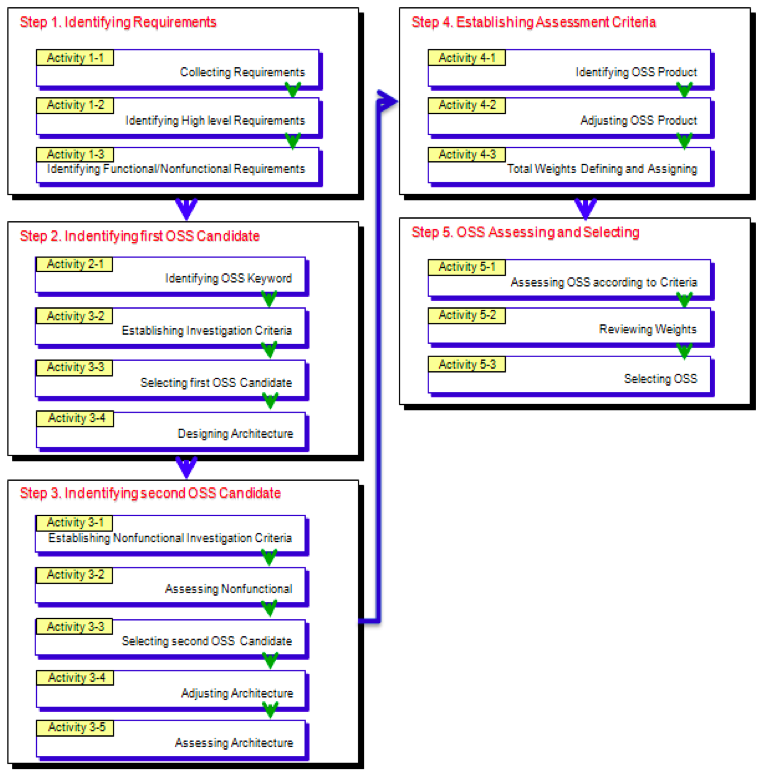
\includegraphics[width=0.5\textwidth ]{img/selectionprocess.png}{}
    \centering
    \caption{Selection Process of OSS. \citet{lee2007study}}\label{fig:selection-process.png}
\end{figure}

\subsection{Source Quality Observatory for Open Source Software}

The SQO-OSS model by \citet{samoladas2008sqo} is focusing on automated software quality assurance. This enables an automatic metrics collection approach and thereby a continuous quality monitoring system can be established which can be seen in Chapter \ref{sec:automated-quality-assurance}. It also takes the community factors into account if only those community factors that can be measured automatically. Next these two community factors it also focuses on the fundamental aspects of open source software quality like the project maintainability, reliability and security.

This model is subdividing every criteria until it is automatically measurable by analyzing source code factors and community attributes. Figure \ref{fig:sqs-oss} is showing the different levels of quality criteria with each subdivision for the specific measurement. Metrics defined by \citet{samoladas2008sqo} are for example for the criteria Changeability: Average size of statements, Vocabulary frequency, Number of unconditional jumps, Number of nested levels, Coupling between objects (CBO), Lack of cohesion (LCOM) and Depth of inheritance tree (DIT). On the community side the metrics for example of the criteria Maturity are: Number of open critical bugs in the last 6 months and Number of open bugs in the last six months. The measurement for this criteria are specified in categories Excellent (E), Good (G), Fair (F) and Poor (P). \citep{samoladas2008sqo}

\begin{figure}[ht]
    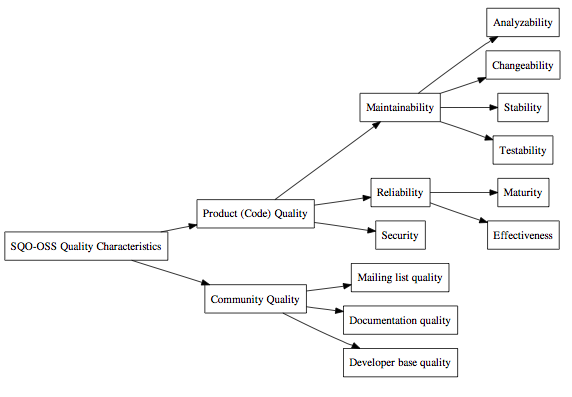
\includegraphics[width=0.5\textwidth ]{img/sqsoss.png}{}
    \centering
    \caption{The SQS-OSS quality model. \citet{samoladas2008sqo}}\label{fig:sqs-oss}
\end{figure}

\subsection{Comparison Framework for Open Source Software Evaluation Methods}

Now the important question is, how to choose between all the different evaluation methods. \citet{stol2010comparison} have already shown the 20 different evaluation methods. They also show if these method comes from industry or research and if it provide a well-defined procedure for applying or not. Next to these information they also offering a framework to compare these evaluation methods.

They call it Framework Framework fOr Comparing Open Source Software Evaluation Methods (FOCOSEM). The following list of metrics are a short overview of this Framework

\begin{enumerate}
    \item Method Context
    \begin{enumerate}
        \item Specific goal: What is the particular goal of the method?
        \item Functionality evaluation: Is functionality compliance part of the evaluation method?
        \item Results publicly available: Are evaluations of OSS products stored in a publicly accessible repository?
    \end{enumerate}
    \item Method User
    \begin{enumerate}
        \item Required skills: What skills does the user need to use the method?
        \item Intended users: Who are the intended users of the method?
    \end{enumerate}
    \item Method Process
    \begin{enumerate}
        \item Method's activities: What are the evaluation method's activities and steps? 
        \item Number of criteria: How many criteria are used in the evaluation?
        \item Evaluation categories: What are the method's categories of criteria based on which the OSS product is evaluated?
        \item Output: What are the outputs of the evaluation method?
        \item Tool support: Is the evaluation method supported by a tool?
    \end{enumerate}
    \item Method Evaluation
    \begin{enumerate}
        \item Validation: Has the evaluation method been validated?
        \item Maturity stage: What is the maturity stage of the evaluation method?
    \end{enumerate}
\end{enumerate}

\enquote{We note that the objective of FOCOSEM is not to make any judgments about different OSS evaluation methods. Instead, we aim to provide insights that may help practitioners to select a suitable OSS evaluation method.} \citep{stol2010comparison}

\section{Automated Quality Assurance\label{sec:automated-quality-assurance}}



% "When developers evaluate the reusability of a component, they often check some of the issues in the project issue tracker and look for signs of activity. Conversely, when developers feel that they have no recourse when defects are found in a reusable component, they are likely to cease reusing it." \citep{Robbins02adoptingoss}


\bibliography{library}

\end{document}
